\documentclass{scrartcl}

\usepackage{siunitx}
\usepackage{graphicx}
\usepackage{caption}
\usepackage{glossaries}
\usepackage[english]{babel}
\usepackage{booktabs}
\usepackage[linktoc=all,hidelinks]{hyperref}
\usepackage{fontspec}
% \usepackage{authblk}
\usepackage{unicode-math}

% \makeatletter
% \renewcommand\AB@affilsepx{,~ \protect\Affilfont}
% \makeatother

\setkomafont{author}{\sffamily}

\newcommand{\nump}[2]{\num[round-mode=places,round-precision=#2]{#1}}
\DeclareGraphicsExtensions{.pdf,.eps}
\bibliographystyle{unsrt}

\title{Report}
\subtitle{A study of machine learning algorithms for reconstruction of missing energy in high energy physics experiments.}
% \subject{Statistical Machine Learning}

\author{
  Max Isacson, \url{max.isacson@physics.uu.se}
  \and
  Mikael M\aa rtensson, \url{mikael.martensson@physics.uu.se}
  \and
  Camila Rangel Smith, \url{camila.rangel@physics.uu.se}
  \and
  Henrik Öhman, \url{ohman@cern.ch}
}
% \author[1]{Max Isacsson}
% \author[2]{Mikael M\aa rtensson}
% \author[3]{Camila Rangel Smith}
% \author[4]{Henrik \"{O}hman}
% \affil[1]{\small\url{max.isacsson@physics.uu.se}}
% \affil[2]{\url{mikael.martensson@physics.uu.se}}
% \affil[3]{\url{camila.rangel@physics.uu.se}}
% \affil[4]{\url{ohman@cern.ch}}

\newacronym{ANN}{ANN}{Artificial Neural Network}
\newacronym{ML}{ML}{Machine Learning}

\newcommand{\etmiss}{$E_\mathrm{T}^\text{miss}$}
\newcommand{\exmiss}{$E_x^\text{miss}$}
\newcommand{\eymiss}{$E_y^\text{miss}$}
\newcommand{\pt}{\ensuremath{p_\text{T}}~}
\newcommand{\mt}{\ensuremath{M_\text{T}}~}

\begin{document}
\maketitle

% \begin{figure}
%     \centering
%     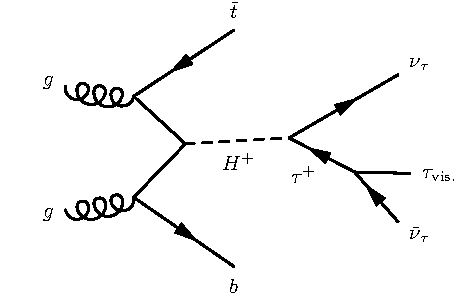
\includegraphics[width=.7\textwidth]{fig/heavyHplustaunu4fs.pdf}
%     \caption{Feynman diagram of the production and decay of a charged Higgs boson. Not shown is the hadronic top decay $\bar t \to \bar b W^-(q \bar q')$.}\label{fig:hplus}
% \end{figure}

\section{Introduction and Objective}

High energy physics experiments have to deal with the so-called "missing energy", which refers to energy coming from particles that do not interact with the particle detector. This particles are usually weakly interacting neutrinos, but it could also come from physics beyond the Standard Model.

This missing energy is estimated by requiring conservation of energy an momentum in the system, and is reconstructed in the transverse plane.  Although this quantity is generally attributed to undetected particles, apparent missing energy may also be caused by mis-measurement on the energy/momentum of the detected particles, this affects the precision on the measurement of the truth missing energy coming from undetected particles. 

In this project we plan to improve the reconstruction of the missing energy by predicting the real contribution from undetected particles. Having a more precise measurement of these contributions could improve the sensitivity of physics to new physics that could be observed in the Large Hadron Collider. 

\section{The Dataset}
\subsection{Structure}
The dataset consists of simulated $pp$ collision events, in which a charged Higgs is produced and decays as $H^+\to\tau\nu$. Each event is described by one set of observable variables and one set of unobservable variables.

Observable variables:
\begin{itemize}
    \item \exmiss, \eymiss --- The $x$- and $y$-components of the missing energy.
    \item $P_{\tau_\mathrm{vis.}}$ --- The 4-momentum of the visible (hadronic) part of the $\tau$ decay.
    \item $P_{b_0}$, $P_{b_1}$, $P_{q_0}$, $P_{q_1}$ --- The 4-momenta of the two $b$-jets and two light jets.
\end{itemize}

Unobservable variables:
\begin{itemize}
    \item $P_{\nu_\tau}$ --- The 4-momentum of the neutrino from the charged Higgs decay.
    \item $P_{\bar\nu_\tau}$ --- The 4-momentum of the neutrino from the $\tau$ decay.
    \item For simplicity, in this particular study it is assumed that the contribution from the neutrino from the $\tau$ decay to the total missing energy is negligible, and only focus on the neutrino from the charged Higgs decay as the unobserved variable. 
\end{itemize}

\subsection{Production}
\texttt{MG5\_aMC@NLO} \cite{Alwall:2014hca} is used for the matrix element computation of $gg / q \bar q \to H^+$ and the event simulation. The events are then passed to \texttt{PYTHIA8} \cite{Sjöstrand2015159} for the showering and hadronization, and for the $H^+\to \tau\nu$ decay. Finally, the detector response is simulated using \texttt{DELPHES} \cite{Favereau2014} with an ATLAS-like geometry.

\subsection{Estimated and true quantities}
The true quantities for both the observable and the unobservable variables are available as output from the event simulation. The estimated values for the observable variables are reconstructed from the output from the detector response simulation.

\section{Methods and Implementation}

\subsection{Strategy}
The neutrino originating from the decay of the Higgs boson will carry the major part of the missing energy in the events. We can approximate the missing transverse energy (\etmiss) by the true transverse momentum (\pt) of the neutrino from the Higgs boson decay. By using this quantity as the target parameter for the training, we aim to find a better estimate of the missing transverse energy. This will result in increased discriminating power of signal from background, since the variables used for discrimination are strongly dependent on this quantity.

\subsection{Feature selection}
In order to select the variables that bring most information into the training, a feature selection was performed based on the p-value of each feature with respect to the target. The best variables in this case are the following:

\begin{itemize}
    \item \exmiss, \eymiss.
    \item $P_{\tau_\mathrm{vis.}}$ 
     \item $P_{b_0}$, $P_{q_0}$, $P_{q_1}$ .
     \item Number of reconstructed $b$-jets in the event.
\end{itemize}

All algorithms presented in this section use these features as inputs in the prediction of the transverse momentum from the neutrino.

\subsection{Regression optimization}
\label{sec:optimization}
For all methods in the following a simple scheme is used to optimize their hyperparameters. We want to predict the \pt\ of the $τ$ neutrino coming from the Higgs boson decay, and the corresponding reconstructed quantity that we want to compare with is the missing transverse energy \etmiss. In order to judge the quality of the prediction we use two figures of merit:
\begin{itemize}
  \item the resolution of the predicted neutrino \pt\ compared to the resolution of the \etmiss, where the resolution is defined as $\frac{x-\pt_ν^{\text{truth}}}{\pt_ν^{\text{truth}}}$, and $x$ is $\pt_ν^{\text{predicted}}$ or \etmiss
  \item the shape of the predicted neutrino \pt\ compared to the true neutrino \pt and the \etmiss; we want the shape to "make physical sense"
\end{itemize}

\subsection{Bayesian Ridge Regression}

A simple approach using linear regression techniques to predict the neutrino transverse moment was investigated. The algorithm with best performance is the Bayesian Ridge Regression, which introduces a zero mean spherical gaussian governed by a single precision parameter as prior probability distribution over the model parameters. The prior and noise parameter are estimated jointly during the fit to the data in several iterations. For an optimal result, 200 iterations are performed, it is found that a larger number of iterations does not improve the prediction.

The result presented here uses \texttt{Python} with \texttt{Numpy} \cite{numpy}, and \texttt{Pandas} \cite{pandas} for general data processing, and \texttt{scikit-learn} \cite{scikit-learn} for the implementation of the algorithm.


\subsection{Artificial Neural Network}

An \gls{ANN} was used to predict the transverse momentum of the neutrino from the charged Higgs decay from the four-momenta of the detected decay products. 
% An \gls{ANN} consists of one input layer, several hidden layers, and an output layer. The input layer consists of the input data vector. The values of this vectors are muliplied by weight and passed on to the hidden layers, where an activation function is applied. In the end, the 

The \gls{ANN} implemented here uses \texttt{Python} with \texttt{SciPy} \cite{scipy}, \texttt{Numpy} \cite{numpy}, and \texttt{Pandas} \cite{pandas} for general data processing, and \texttt{Keras} \cite{keras} for the actual neural network. The number of input nodes is restricted to the 19 selected predictor variables and the output to the target dimension of 1. Since the network is used for regression, the activation functions between the last hidden layer and the output must be linear.

The data is scaled to avoid the tails of the \gls{ANN} activation functions and improve the learning rate. The method used here is to scale it such that the minimum is -1 and the maximum is 1 for each training set variable. The test set data is scaled using the scaling parameters computed from the training set. Another scaling method is to scale the mean to 0 and the standard deviation to 1, but this was found to slow down the training and give worst results.

Training is performed using stochastic gradient descent with the Nesterov method \cite{nesterov} and a mean-squared-error loss function. The learning rate was set to 0.1, the learning rate decay to $\num{1e-6}$, and the momentum to 0.9.

A large number of configurations of the hidden layers were tested by varying the number of layers, the number of perceptrons in each layer, and the activation functions (sigmoid, tanh, and softmax). Sigmoid activation functions produced the best result for a fixed training period. A network with two hidden layers (i.e. 4 layers counting the 19 node input layer and 1 node output layer) with 25 and 10 perceptrons was found to be sufficiently complex. Using deeper networks, e.g. one with 4 hidden layer with 20, 35, 25, and 15 perceptrons, did not improve the result.

\subsection{Support Vector Regression}

Support vector machines can be used for regression, and the method is then called support vector regression (SVR). It employs two slack variables, $ξ_n ≥ 0$ and $\hat{ξ}_n ≥ 0$ and the corresponding error function to minimize is
\[
  C \sum_{n=1}^N(ξ_n + \hat{ξ}_n) + \frac{1}{2}||w||^2
\]
where $C$ is the cost variable. The implementation used is the \texttt{SVR} class from \texttt{scikit-learn}, and it is an $ε$-SVR method. This implementation has four built-in kernels: RBF, sigmoid, linear, and polynomial. The selected predictors in the dataset are scaled to have a mean of 0 and a variance of 1 using the \texttt{StandardScaler} class from \texttt{scikit-learn}.

With the presented dataset, the selected SVR algorithm is not converging within a few minutes runnning time. The maximum number of iterations is therefore limited to 1000. A greater number of iterations is not found to yield significantly better results. The kernel that performs best is the RBF kernel. The value of the cost function is by default set to 1.0, but this setting yields a very poor resolution. Different values of the cost function are tested, and a value of $C=100.0$ is found to be (near) optimal. For the soft margin the default value of $ε=0.1$ is good.

Regardless of the choice of $C$ and $ε$, the performance of the SVR is found to be no better than that of linear ridge regression. The resolution is not improved, and the shape of the true and reconstructed transverse component of the missing energy is not recovered by the prediction.

\subsection{Trees and forests}

Decision trees and ensemble methods, and in particular boosted decision trees (BDTs), have been a popular choice of method in particle physics. The method of decision trees are based on using multiple discriminating variables, and multiple choices in a binary tree, to find the prediction that best describes the target variable. When using ensemble methods, such as extra trees, gradient boosting, or random forests multiple such trees are created, each with its own weight describing its "importance". The tree depth plays an important role when considering the trade-off between over-training and bias, and with the ensemble methods the number of trees is also an important parameter.

The performances of the classes \texttt{DecisionTreeRegressor}, \texttt{ExtraTreesRegressor}, \texttt{GradientBoostingRegressor}, and \texttt{RandomForestRegressor} in \texttt{scikit-learn} are examined. Different settings for the tree depth and (for the ensemble methods) number of trees are used. Near optimal values for the depth and the number of trees is found to be 15 and 100 for all methods and all ensemble methods respectively. The decision tree regression shows some improvement in resolution, but the shape of the transverse component of the missing energy is not recovered by the prediction. Neither in the ensemble methods is the shape of the missing energy recovered, but the resolution is improved. All three ensemble method show similar performance.

\subsection{Gaussian process regression}
Formally, a Gaussian process is a stochastic process defined as a probability distribution over functions $y(\mathbf x)$, such that a set of function values $y_1, \ldots, y_N$ evaluated at inputs $\mathbf x_1, \ldots, \mathbf x_N$ are jointly Gaussian distributed.

Given a training data set of targets $\mathbf t = (t_1,\ldots,t_N)^\text{T}$ corresponding to inputs $\mathbf x_1,\ldots,\mathbf x_N$, regression can be performed on the new target $t_{N+1}$ given new input $\mathbf x_{N+1}$ by calculating the conditional probability $p(t_{N+1}|\mathbf t)$. This will be a Gaussian distribution with mean and covariance given by
\begin{align}
    m(\mathbf x_{N+1}) &= \mathbf k^\text{T} \mathbf C^{-1}_N \mathbf t \\
    \sigma^2(\mathbf x_{N+1}) &= c - \mathbf k^\text{T} \mathbf C^{-1}_N \mathbf k
\end{align}
where the elements of $\mathbf C$ are $C_{nm} = k(\mathbf x_n, \mathbf x_m) + \beta^{-1}\delta_{nm}$, the elements of $\mathbf k$ are $k_n = k(\mathbf x_n, \mathbf x_{N+1})$, and $c = k(\mathbf x_{N+1}, \mathbf x_{N+1}) + \beta^{-1}$. Here $k(\mathbf x, \mathbf x')$ is the kernel function, and $\beta$ is the precision of the noise in the measurements, assuming that the noise $\epsilon_n$ for each measurement is isotropically distributed as $\mathcal N(\mathbf 0 | \beta^{-1}\mathbb 1)$.

The squared exponential was choosen as the kernel method, defined by
\begin{equation}
    k(\mathbf x, \mathbf x') = \exp( -\theta ||\mathbf x - \mathbf x'||^2 )
\end{equation}
where the parameter $\theta$ is estimated using maximum likelihood, and is allowed to float between $10^{-4}$ and $10^{-1}$. The precision of the noise was taken as $\beta = 100$. 

Training and testing of the Gaussian processes was done using 3-fold cross validation on 8000 measurements. Due to the non-sparseness of Gaussian processes and memory constraints, more data than this was not feasible to use in the training.
\section{Results}
\label{sec:results}

The final metrics to measure the performance of the algorithms are the resolution (as described in Section~\ref{sec:optimization} above), the ratio of the predicted value with respect to its true value, and the transverse mass of the $τ$ and neutrino system. The transverse mass $\mt$ is defined as:
\begin{equation}
  \label{eq:mt}
  \mt=\sqrt{ 2 \pt^\tau \pt^\nu   (1-\cos \Delta\phi_{\tau,\text{miss}}) },
\end{equation}
where $\Delta\phi_{\tau,\text{miss}}$ is the azimuthal angle between the $\tau$ and the direction of the missing transverse momentum. 

% Please describe how the missing mass is calculated

\section{Discussion}

This project focused on predicting the transverse momentum \pt of the neutrino from the charged Higgs decay by using the reconstructed four-momenta of the detected particles and the missing energy as inputs and training on the true \pt given by the Monte-Carlo simulation.

Out of all the \gls{ML} methods tried, \gls{ANN} and the bayesian ridge regression showed the best performance. The  \gls{ANN} shows the smallest bias in resolution with respect to the Bayes ridge regression but observes a significantly worse variance. All methods show a narrower transverse mass distribution, which is beneficial to discriminate signal over backgrounds.

The mass of the $H^+$ is the ultimate discriminant variable, but is not built due to the lack of longitudinal information in the detector, one option would be is to target the $H^+$ mass directly and complement the missing information. This would require Monte-Carlo for a range of possible $H^+$ masses (3 mass-points were used in this study) and well for the background events. 

As stated before, in this project it is assumed that the contribution from the neutrino from the $\tau$ decay to the total missing energy is negligible, and only focus on the neutrino from the charged Higgs decay as the unobserved variable. This approach is not correct for higher masses of the $H^+$. A more complete study would be to target the complete three-vector of the missing energy or the (combined or separate) four-vectors of the two neutrinos. These options were briefly looked at but were considered to be out of the scope of this project. They will be pursued in more detail in future studies.

% ISN'T THIS LAST PARAGRAPH THE SAME AS THE PREVIOUS ONE? OF RECONSTRUCTING THE 3-VECTOR? THIS PARAGRAPH IS A BIT CONFUSING.
% To compute the missing transverse mass \mt (described in sec. \ref{sec:results}) from the \pt predicted by the \gls{ML} methods, the angle $\phi$ of the \pt is needed. However, since we are only predicting the \pt, the angle $\phi$ is unknown and is instead taken from the angle of \mt. It would have been better to also predict $\phi$. This will also be studied in the future.

% Mention that we use phi(met) when calculating the mT for the prediction. In principle we should predict phi as well. 
% The second nu as source of error

\bibliography{refs}

\end{document}
